\documentclass[a4paper,12pt]{article}

\usepackage{fontspec}
\newfontfamily{\defaultfont}{CMU Serif}
\newfontfamily{\thaifont}[Scale=MatchLowercase]{TH Sarabun Chula}

\usepackage{polyglossia}
\setdefaultlanguage{thai}
\setotherlanguages{english}

\usepackage[Latin,Thai]{ucharclasses}
\setDefaultTransitions{\defaultfont}{}
\setTransitionTo{Thai}{\thaifont}

\XeTeXlinebreaklocale "th"
\XeTeXlinebreakskip = 0pt plus 0pt

\linespread{1.25}

\usepackage{amsmath,amsthm,amssymb}
\usepackage[ISO]{diffcoeff}
\usepackage{siunitx}
\usepackage[margin=1in]{geometry}
\usepackage{graphicx}
\usepackage{hyperref}
	
\title{Lagrangian Mechanics ฉบับพื้นฐาน}
\author{อิธิพัฒน์ ธนบดีกาญจน์}

\begin{document}

\renewcommand{\thefootnote}{\fnsymbol{footnote}}

\maketitle

\section{บทนำ}
Lagrange Mechanics เป็นการบรรยายการเคลื่อนที่ของวัตถุต่าง ๆ โดยอาศัยพลังงานและ Principle of Stationary Action ซึ่งแตกต่างจาก Newtonian Mechanics ที่อาศัย “แรง” บรรยาย ทำให้มีจุดเด่นในการแก้ปัญหาที่มีวัตถุหรือองศาเสรี (Degree of Freedom) จำนวนมากเพราะปริมาณต่าง ๆ ที่พิจารณาเป็นปริมาณสเกลาร์

\section{สมการ Euler–Lagrange}
พิจารณาสถานการณ์ที่เราต้องการหาสมการบรรยายการเคลื่อนที่แล้วตีตารางลงบนสถาณการณ์นั้น
\begin{figure}[h]
	\centering
	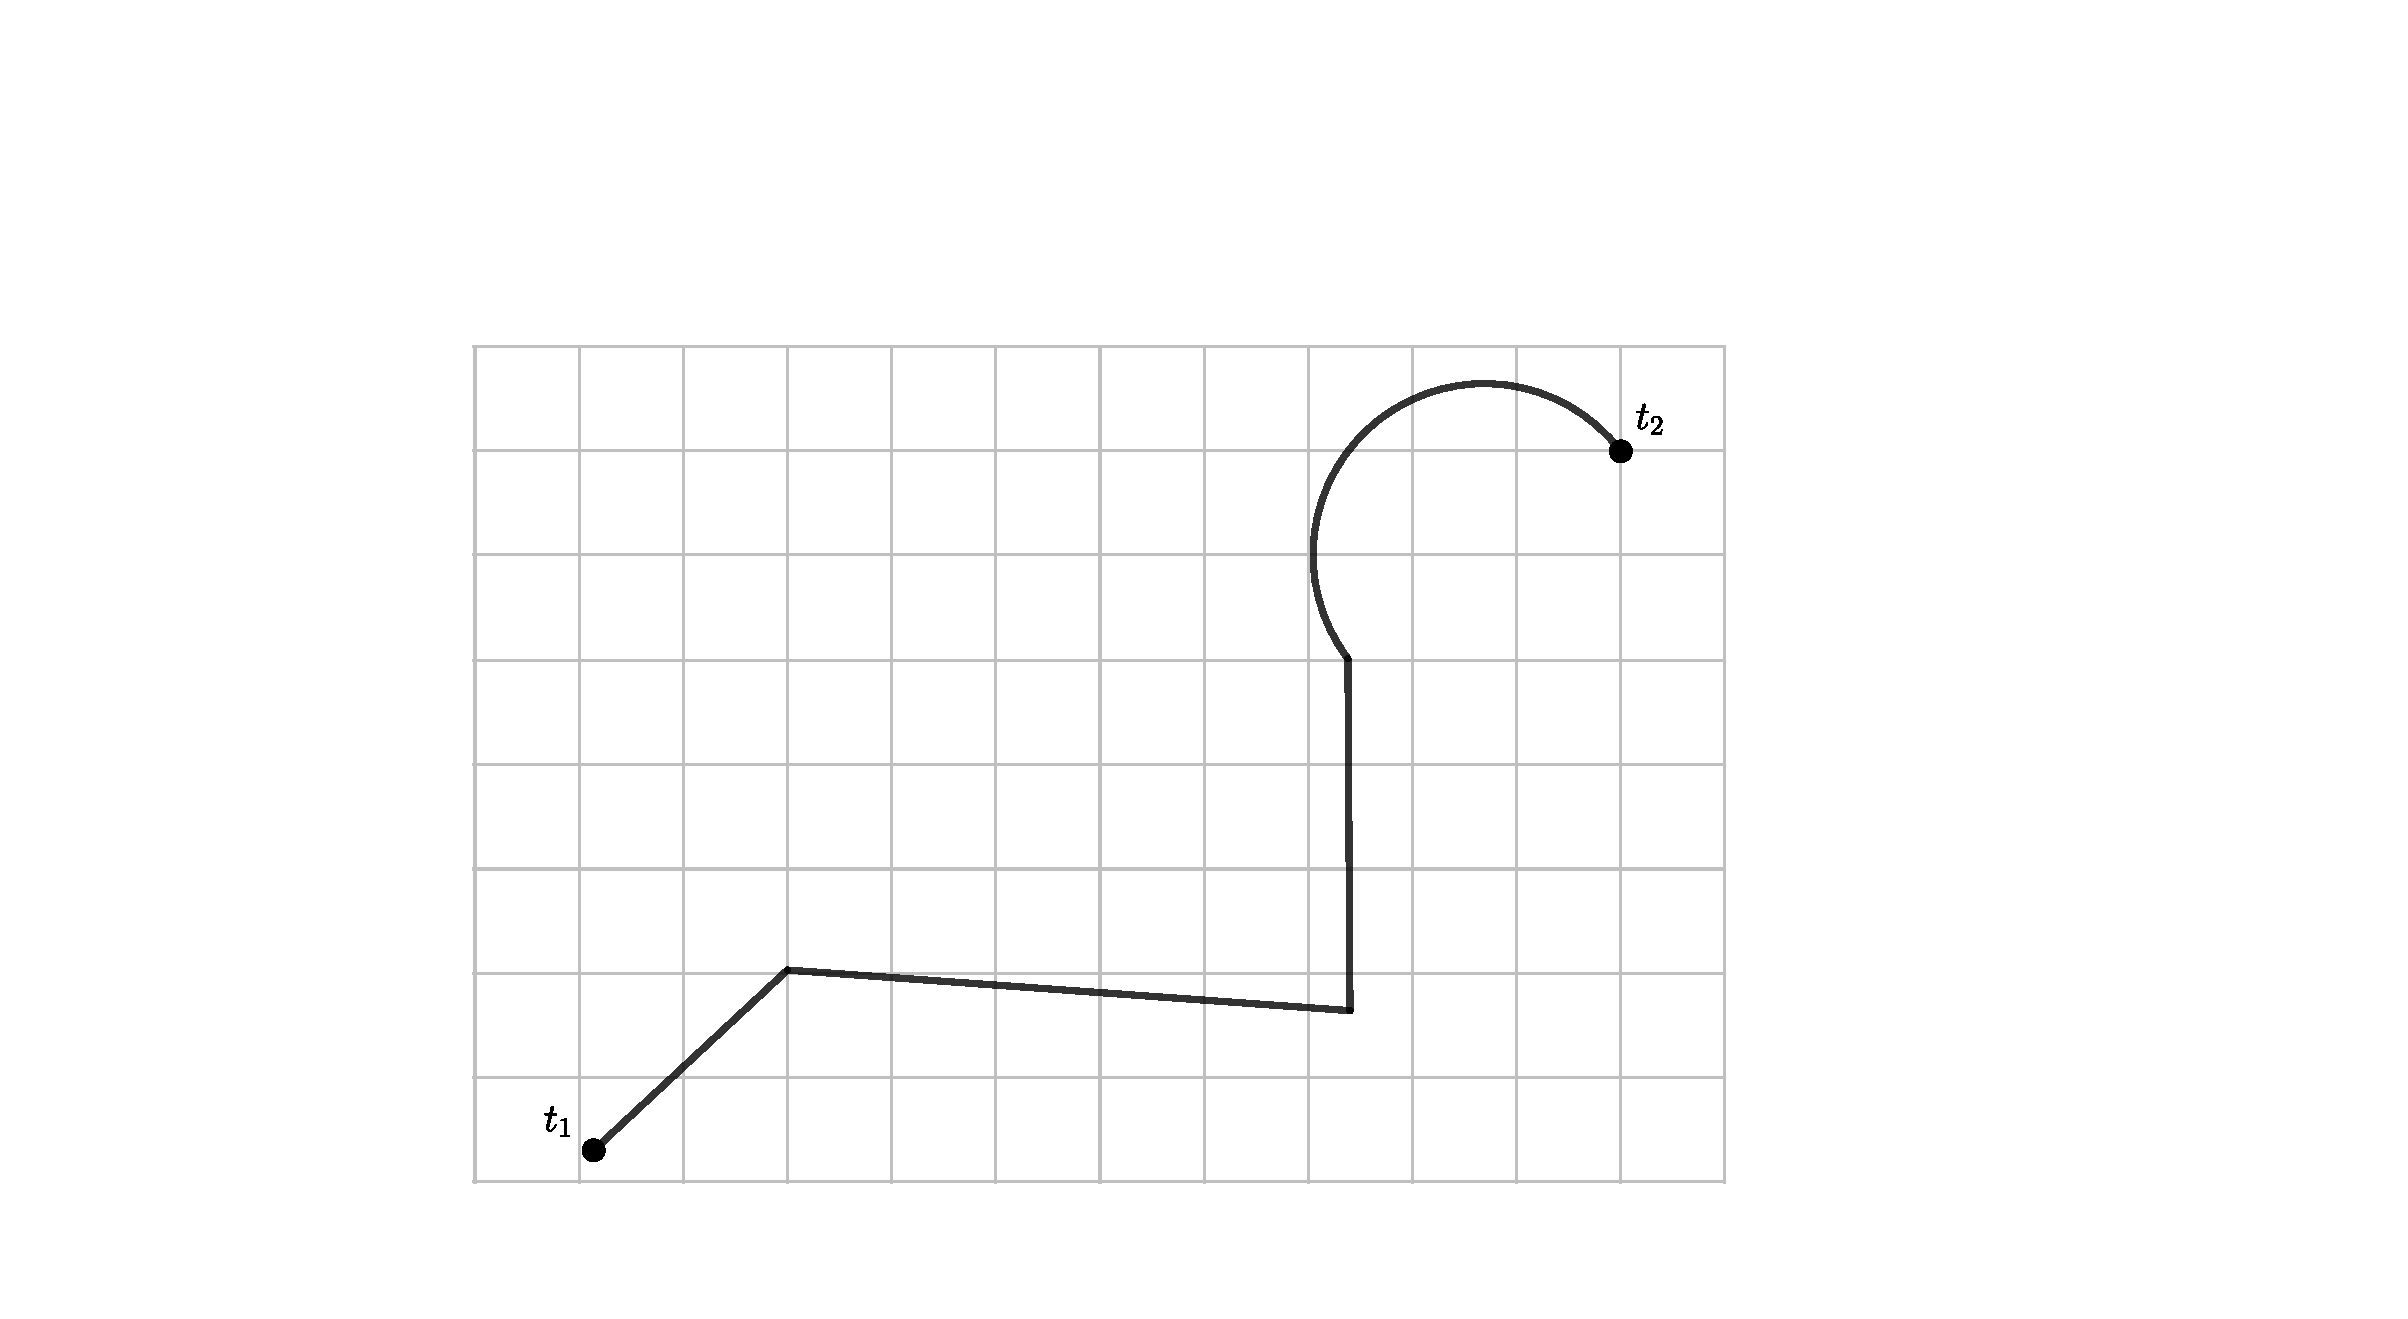
\includegraphics[width=0.7\linewidth]{path}
	\label{fig:path}
\end{figure}
\\จากนั้นหาค่าพลังงานจน์ลบพลังงานศักย์ของทุกช่อง
\begin{figure}[h]
	\centering
	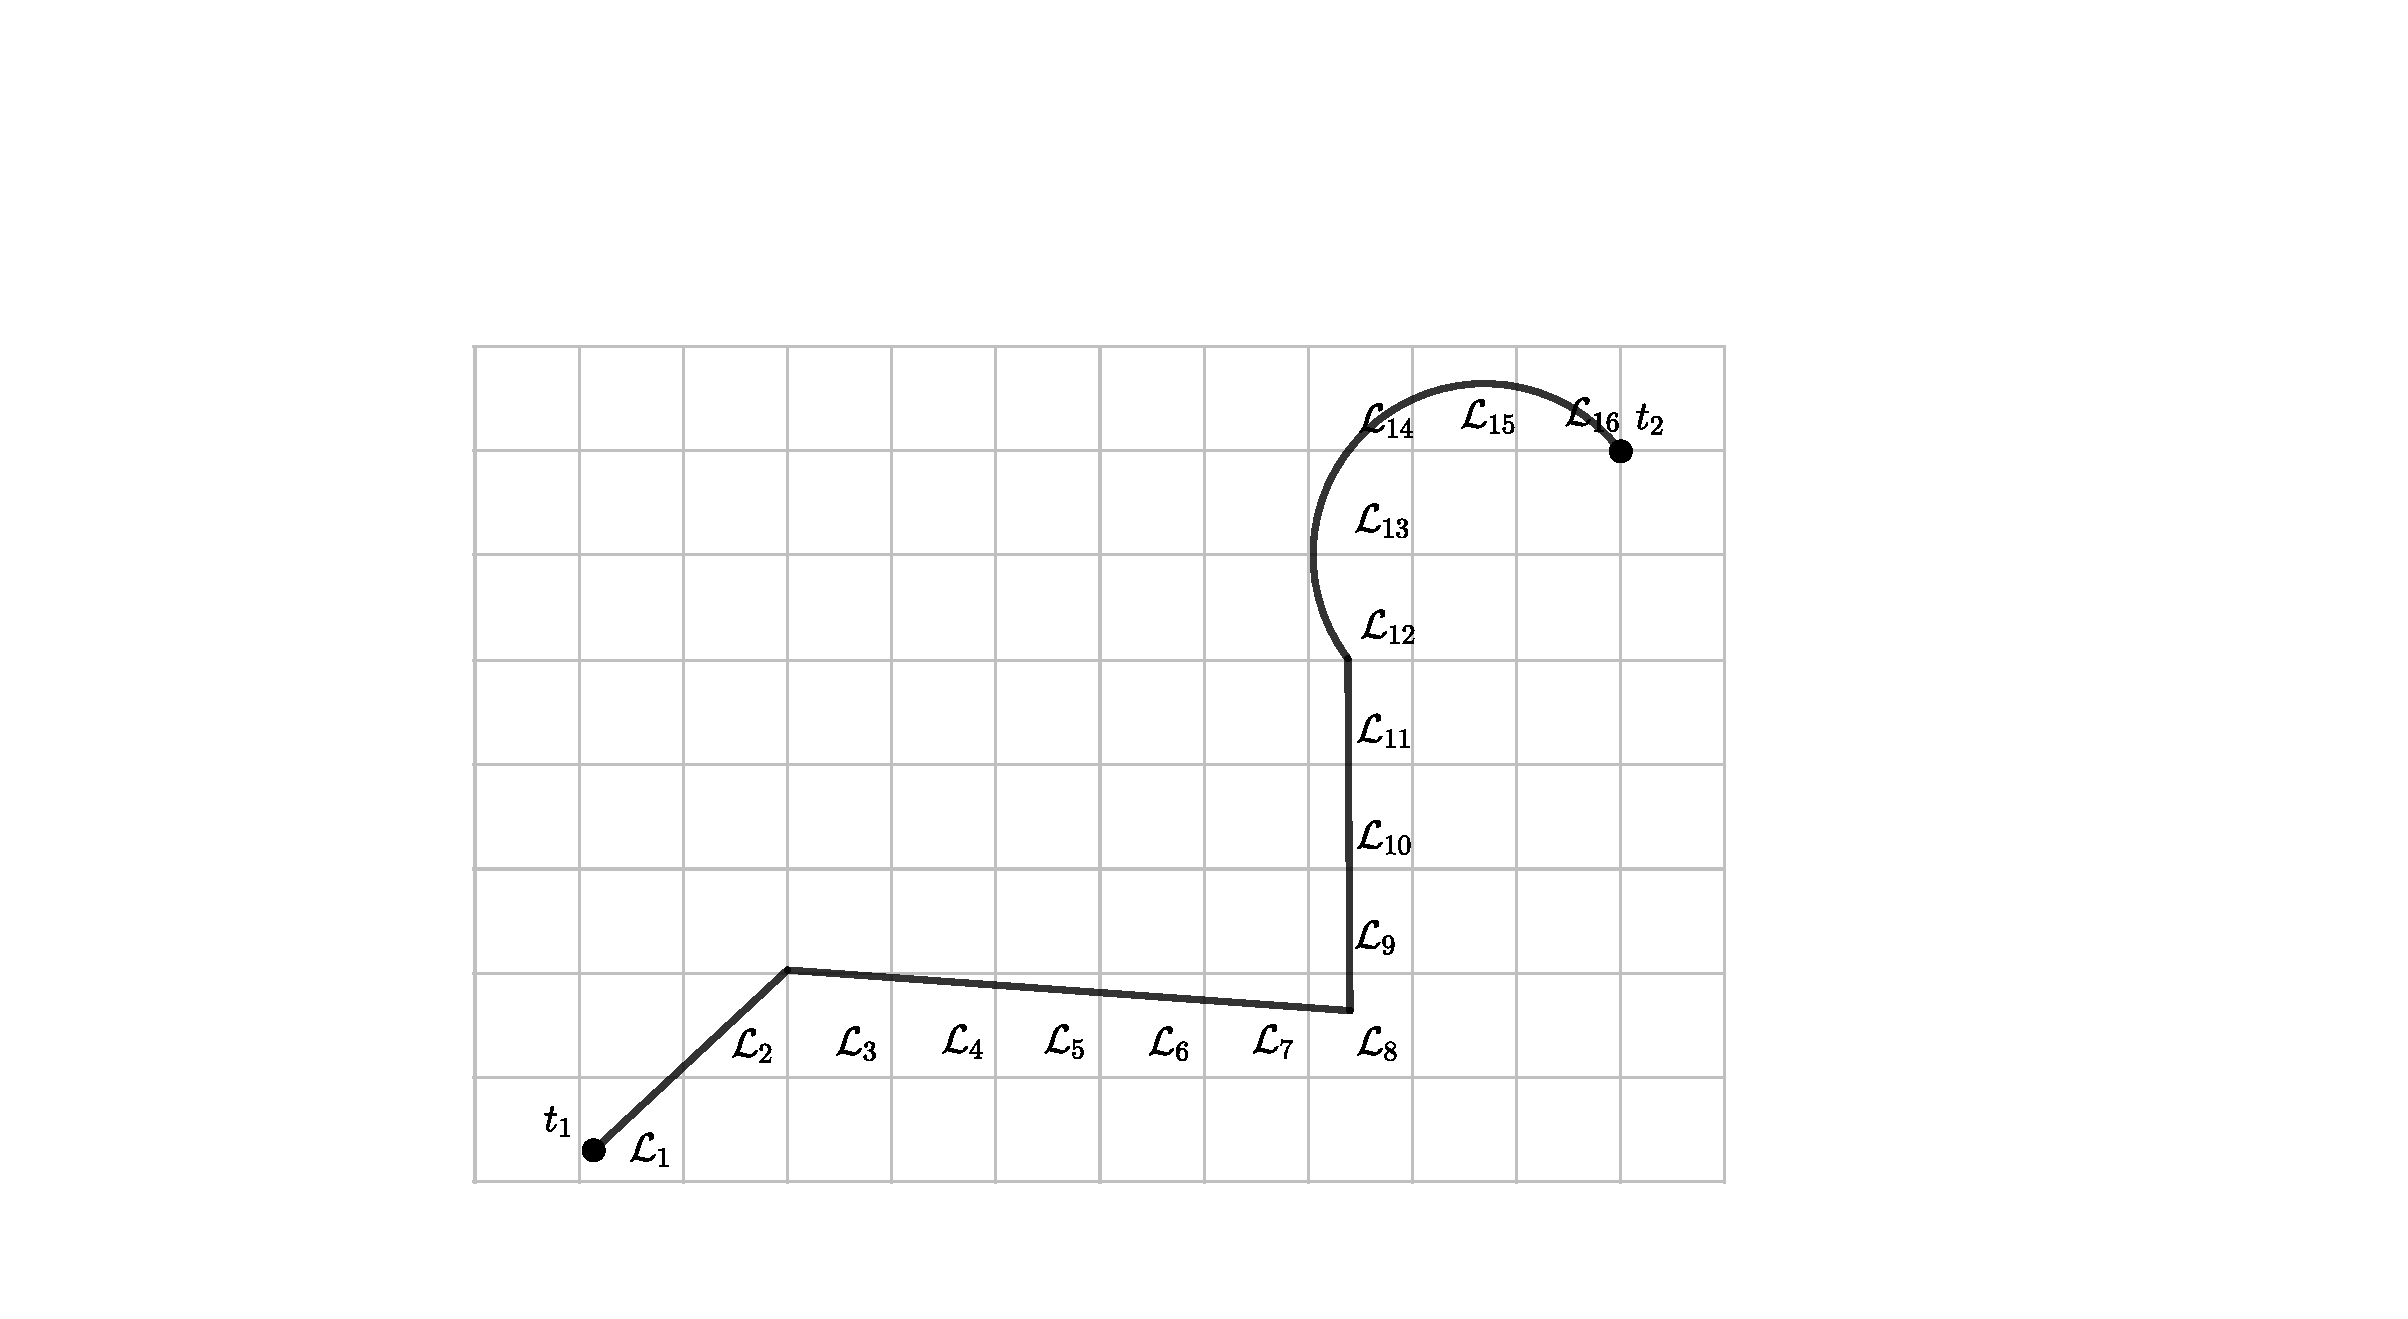
\includegraphics[width=0.7\linewidth]{path_lagrangian}
	\label{fig:pathlagrangian}
\end{figure}
โดยเราจะนิยามค่าในตารางนั้นว่า Lagrangian (\(\mathcal{L}\))
\begin{equation}
	\mathcal{L}\equiv K-U
\end{equation}
เนื่องจากการพิจารณานี้เราทราบว่าวัตถุเริ่มที่เวลาใดและจบที่เวลาใด เราจึงหาผลรวมของ Lagrangian ตามเส้นทางที่วัตถุเคลื่อนที่จากเริ่มต้น (\(t_1\)) จนถึงเวลาที่เราสนใจ (\(t_2\)) โดยรวมระยะเวลาย่อย ๆ ทีละ \(\Delta t\)
\begin{equation*}
	\sum_{t=t_1}^{t_2}\mathcal{L}\Delta t
\end{equation*}
จากนั้นกำหนด \(\Delta t \to 0\) ทำให้ตารางมีความละเอียดเป็นอนันต์และได้ค่าที่เที่ยงตรงไม่ว่าจะเป็นเส้นทางใด ๆ
\begin{equation*}
	\lim_{\Delta t \to 0}\sum_{t=t_1}^{t_2}\mathcal{L}\Delta t
\end{equation*}
เรานิยามค่านี้คือ Action(\(S\)) และเปลี่ยนสัญลักษณ์เป็นปริพันธ์
\begin{equation}
	S\equiv\int_{t_1}^{t_2}\mathcal{L}\,\dl t
\end{equation}
เราทราบว่า \(\mathcal{L}\) ขึ้นอยู่กับ \(K\) และ \(U\) ดังนั้น \(\mathcal{L}\) จะขึ้นอยู่กับ \(x(t)\), \(\dot{x}(t)\) และ \(t\) ด้วย\footnote{เช่น \(K=\frac{1}{2}m(\dot{x}(t))^2\) และ \(U=mgx(t)\)} เราจึงทำการนิยามฟังก์ชันบรรยายการเคลื่อนที่ของวัตถุให้เท่ากับฟังก์ชันคงที่ (\(x_0(t)\)) บวกกับฟังก์ชันที่แปรผันได้ (\(\alpha\beta(t)\)) เพื่อช่วยในการแก้ปัญหานี้
\begin{equation}
	x(t)\equiv x_0(t)+\alpha\beta(t)
	\label{eq:path}\end{equation}
และหาอนุพันธ์เทียบเวลาเพื่อหา \(\dot{x}(t)\)
\begin{equation}
	\dot{x}(t)=\dot{x}_0(t)+\alpha\dot{\beta}(t)
	\label{eq:velocity}\end{equation}
ทั้งนี้การที่มี \(\alpha\) คูณกับ \(\beta\) นั้นจะช่วยทำให้เราสามารถใช้แคลคูลัสหนึ่งตัวแปรแก้ปัญหาได้และ \(\beta(t_1)=0,\beta(t_2)=0\) เพราะเรากำหนดให้ต้นทางเริ่มที่ \(x(t_1)\) และ \(x(t_2)\) แต่เส้นทางการเคลื่อนที่ยังคงเปลี่ยนแปลงได้\\
จาก Principle of Stationary Action จะได้
\begin{align*}
	\diff{S}{\alpha}                                   & =0 \\
	\diff*{\int_{t_1}^{t_2}\mathcal{L}\,\dl t}{\alpha} & =0
\end{align*}
อาศัย Leibniz Integral Rule จะได้
\begin{equation*}
	\int_{t_1}^{t_2}\diffp{\mathcal{L}}{\alpha}\,\dl t=0
\end{equation*}
ระลึกว่า \(\mathcal{L}\) เป็นฟังก์ชันที่ขึ้นกับ \(x(t)\), \(\dot{x}(t)\) และ \(t\) อาศัย Chain rule จะได้
\begin{equation}
	0=\int_{t_1}^{t_2}\diffp{\mathcal{L}}{x}\diffp{x}{\alpha}+\diffp{\mathcal{L}}{\dot{x}}\diffp{\dot{x}}{\alpha}+\diffp{\mathcal{L}}{t}\diffp{t}{\alpha}\,\dl t
	\label{eq:partial}\end{equation}
หาอนุพันธ์ย่อยเทียบ \(\alpha\) ของสมการ (\ref{eq:path}) และ (\ref{eq:velocity})
\begin{align}
	\diffp{x}{\alpha}       & =\beta\label{eq:help1}       \\
	\diffp{\dot{x}}{\alpha} & =\dot{\beta}\label{eq:help2} \\
	\diffp{t}{\alpha}       & =0\label{eq:help3}
\end{align}
นำ (\ref{eq:help1}), (\ref{eq:help2}) และ (\ref{eq:help3}) แทนใน (\ref{eq:partial})
\begin{align}
	0 & =\int_{t_1}^{t_2}\diffp{\mathcal{L}}{x}\beta+\diffp{\mathcal{L}}{\dot{x}}\dot{\beta}\,\dl t \label{eq:partial2}                        \\
	0 & =\int_{t_1}^{t_2}\diffp{\mathcal{L}}{x}\beta\,\dl t+\int_{t_1}^{t_2}\diffp{\mathcal{L}}{\dot{x}}\dot{\beta}\,\dl t \nonumber
\end{align}
จากนั้นเราจะทำ Integration by Parts พจน์หลังเพื่อกำจัด \(\dot{\beta}\)
\begin{equation*}
	0=\int_{t_1}^{t_2}\diffp{\mathcal{L}}{x}\beta\dl t+\left[\diffp{\mathcal{L}}{\dot{x}}\beta\right]_{t_1}^{t_2}-\int_{t_1}^{t_2}\diff*{\left(\diffp{\mathcal{L}}{\dot{x}}\right)}{t}\beta\,\dl t
\end{equation*}
เนื่องจากเรากำหนดให้ \(\beta(t_1)=0\) และ \(\beta(t_2)=0\) ดังนั้น
\begin{align*}
	0 & =\int_{t_1}^{t_2}\diffp{\mathcal{L}}{x}\beta\dl t-\int_{t_1}^{t_2}\diff*{\left(\diffp{\mathcal{L}}{\dot{x}}\right)}{t}\beta\,\dl t \\
	0 & =\int_{t_1}^{t_2}\left(\diffp{\mathcal{L}}{x}-\diff*{\left(\diffp{\mathcal{L}}{\dot{x}}\right)}{t}\right)\beta\,\dl t
\end{align*}
สมการดังกล่าวจะเป็นจริงได้ก็ต่อเมื่อพจน์ในวงเล็บเท่ากับศูนย์เท่ากันเพราะ \(\beta\) ไม่จำเป็นต้องมีค่าเป็นศูนย์ เราจึงสรุปได้ว่า
\begin{equation*}
	\diffp{\mathcal{L}}{x}-\diff*{\left(\diffp{\mathcal{L}}{\dot{x}}\right)}{t}=0
\end{equation*}
เราจะทำให้สมการนี้อยู่ในรูปทั่วไปของระบบที่มี \(N\) องศาเสรีโดยเปลี่ยนตัวแปร \(x\) เป็น \(q\) ตามความนิยมและใช้ตัวดำเนินการ \(\sum\) (เสมือนว่าได้ละตัวดำเนินการ \(\sum\) มาตลอดการพิสูจน์)
\begin{equation}
	\sum_{i=1}^{N}\left( \diffp{\mathcal{L}}{q_i}-\diff*{\left(\diffp{\mathcal{L}}{\dot{q_i}}\right)}{t}\right) =0
\end{equation} 
จาก Fundamental Lemmas of the Calculus of Variations จะได้ว่าทุกพจน์ที่บวกกันต้องเท่ากับ 0 (ระลึกว่าแต่ละพจน์มี \(\beta\) คูณอยู่)
\begin{equation}
	\boxed{\diffp{\mathcal{L}}{q_i}-\diff*{\left(\diffp{\mathcal{L}}{\dot{q_i}}\right)}{t} =0,\quad i=1,2,\dots,N}\label{eq:e-l}
\end{equation} 
เรียกสมการนี้ว่า Euler–Lagrange เนื่องจาก Euler และ Lagrange ได้ร่วมกันแก้ปัญหาดังกล่าว
\section{ตัวอย่างการใช้งานสมการ Euler-Lagrange}
ทรงกระบอกมวล \(m\) รัศมี \(r\) ติดสปริงที่มีค่าคงตัว \(k\) จงหาคาบของการสั่นเมื่อขยับทรงกระบอกแล้วปล่อย ทรงกระบอกกลิ้งแบบไม่ไถล\cite{morin}\\
สังเกตระบบจะพบว่ามีพลังงานศักย์หยืดหยุ่นและพลังงานจลน์เกี่ยวข้อง
\begin{figure}[h]
	\centering
	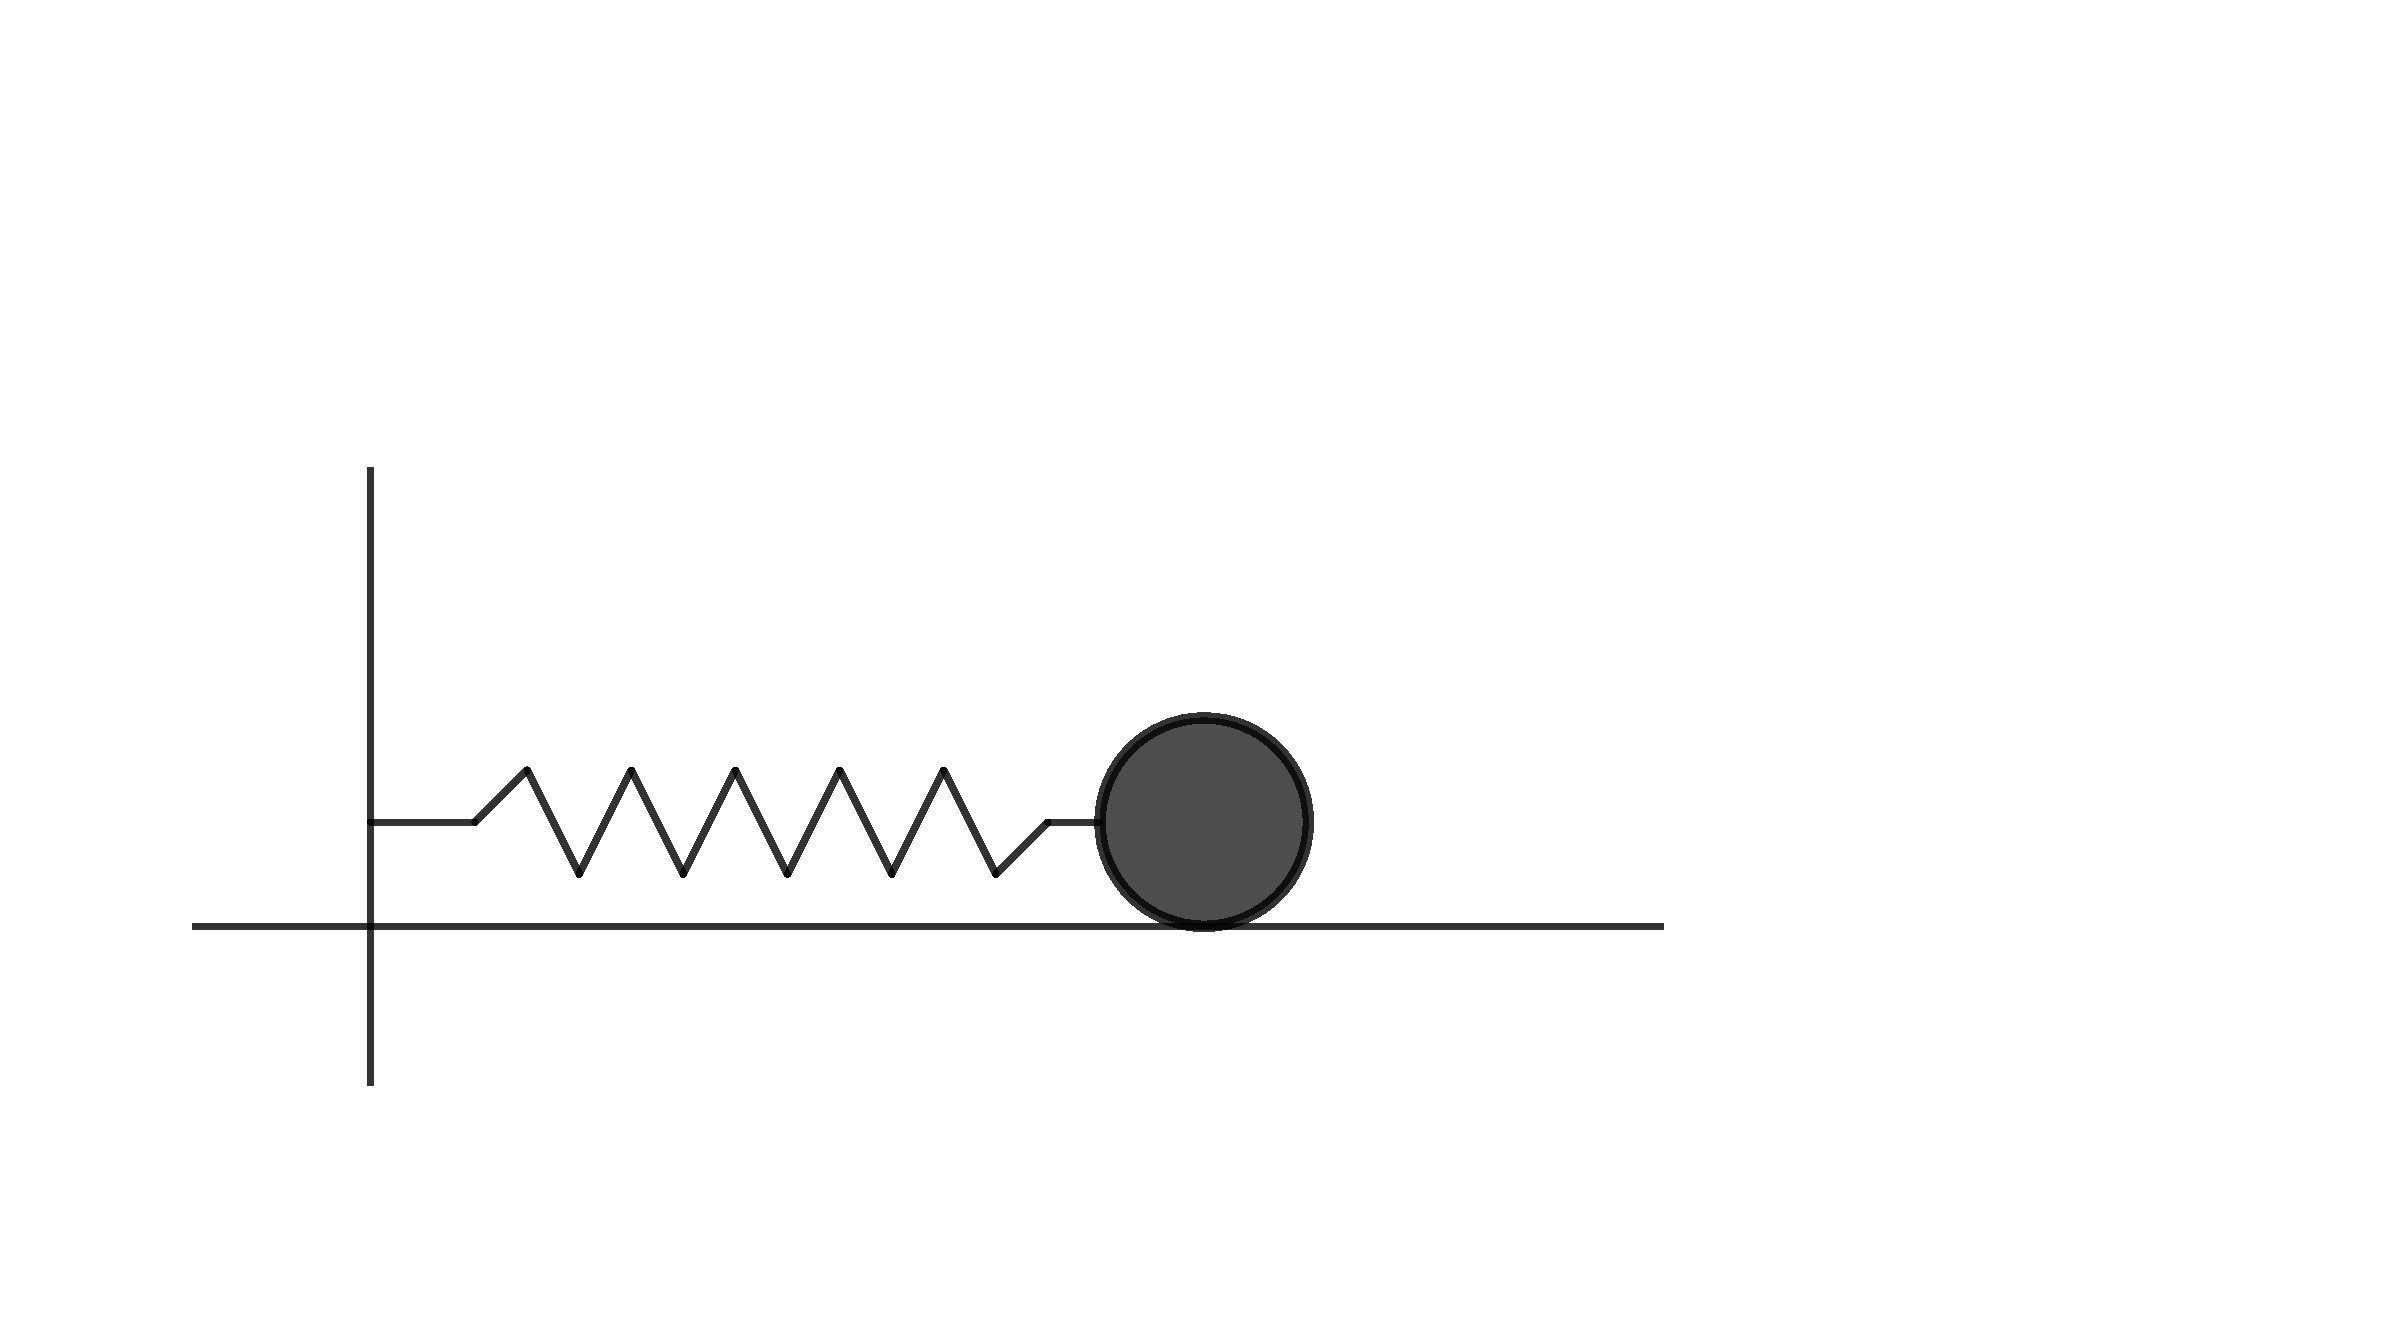
\includegraphics[width=0.4\linewidth]{cylinderrollwithspring}
	\label{fig:cylinderrollwithspring}
\end{figure}\\
จาก
\begin{equation}
	\mathcal{L}=K-U
\end{equation}
ได้
\begin{align}
	\mathcal{L} & =\frac{1}{2}mv^2+\frac{1}{2}I_{\text{CM}}\omega^2-\frac{1}{2}kx^2\nonumber                                                \\
	\mathcal{L} & =\frac{1}{2}m\dot{x}^2+\frac{1}{2}\left( \frac{1}{2}mr^2\right) \left(\frac{\dot{x}}{r}\right)^2-\frac{1}{2}kx^2\nonumber \\
	\mathcal{L} & =\frac{3}{4}m\dot{x}^2-\frac{1}{2}kx^2\label{eq:l1}
\end{align}
นำสมการ (\ref{eq:l1}) แทนไปในสมการ (\ref{eq:e-l})
\begin{align}
	0        & =\diffp*{\left( \frac{3}{4}m\dot{x}^2-\frac{1}{2}kx^2\right)}{x} -\diff*{\left(\diffp*{\left( \frac{3}{4}m\dot{x}^2-\frac{1}{2}kx^2\right) }{\dot{x}}\right)}{t}  \nonumber \\
	0        & =(-kx)-\diff*{\left(\frac{3}{2}m\dot{x}\right)}{t}                                                                                                   \nonumber              \\
	0        & =-kx-\frac{3}{2}m\ddot{x}                                                                                                                           \nonumber               \\
	\ddot{x} & =-\left( \frac{2k}{3m}\right) x\label{eq:newtonshm}
\end{align}
นำสมการ (\ref{eq:newtonshm}) เทียบกับสมการในรูปทั่วไปของ SHM\footnote{\(\ddot{x}=-\omega^2x\)} ดังนั้นจะได้
\begin{equation}
	\omega=\sqrt{\frac{2k}{3m}}\label{eq:omegacylin}
\end{equation}
จาก
\begin{equation}
	T=\frac{2\pi}{\omega}\label{eq:period}
\end{equation}
นำสมการ (\ref{eq:omegacylin}) แทนใน (\ref{eq:period})
\begin{equation*}
	T=2\pi\sqrt{\frac{3m}{2k}}\ \blacksquare
\end{equation*}
\begin{thebibliography}{9}
	\bibitem{morin}
	Morin, D. (2008). \textit{Introduction to classical mechanics: with problems and solutions}. Cambridge University Press.
\end{thebibliography}

\end{document}